\section{Visualization Design}


In this section, we introduce the visual design based on the design tasks discussed in Sec.\ref{section:design_tasks}.  As shown in Fig.~\ref{fig:teaser}, the visual analytic system consists of six coordinated views. Starting from the configuration panel Fig.~\ref{fig:teaser}B, the users are able to select the target feature and the model to be analyzed. The region partition will be shown as Fig.~\ref{fig:teaser}B after the model is selected. To support exploring the model mechanism, the Cluster View is displayed to summarize the hidden units' response to the features (Fig.~\ref{fig:teaser}A) and the Feature Importance View (Fig.~\ref{fig:teaser}C) is shown to visualize the temporal importance of each feature. Furthermore, the users can select the individual cases in the Projection View (Fig.~\ref{fig:teaser}E) and all the selected individual cases are grouped by similarity and displayed in the Individual View (Fig.~\ref{fig:teaser}D).


\begin{figure}[t]
	\centering
	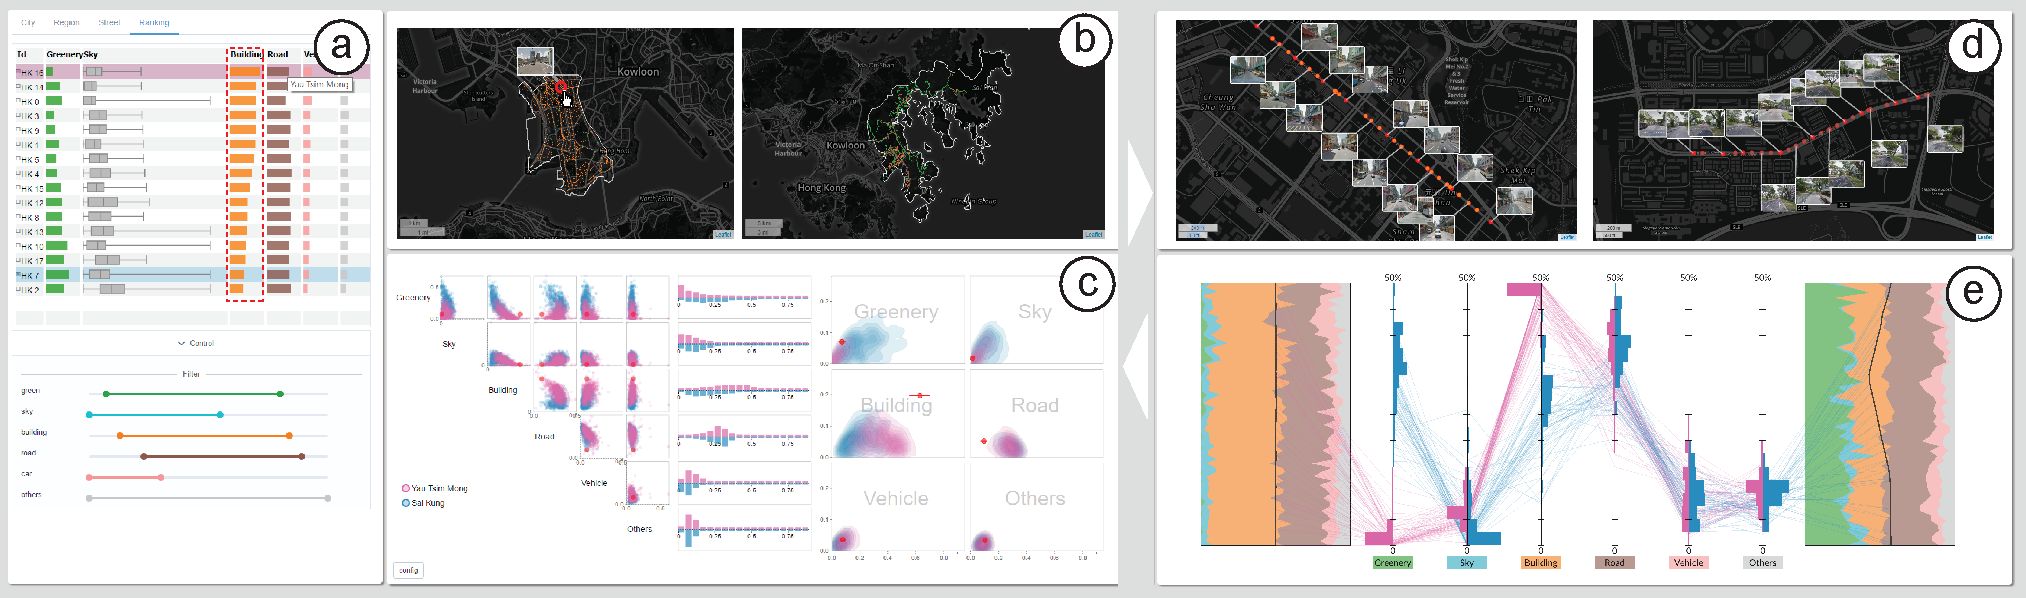
\includegraphics[width=0.95\textwidth]{figure/MultiRNNExplorer/teaser.pdf}
	\vspace{-3mm}
	\caption{Design of Hidden unit distribution and feature glyph. A) Hidden unit cluster; B) Hidden unit distribution; C) Feature cluster; D) Feature distribution for selected features; E) Feature glyph design; G) Response link MultiRNNExplorer contains multiple coordinated views to support exploring and understanding RNNs' behaviors on multi-dimensional time-series data, especially on hidden unit response and feature importance.
		The Configuration Panel (B) allows users to select a RNN models and configure parameters. 
		To reveal model mechanism, the Cluster View (A) summarizes the hidden unit clusters' response to feature clusters, and the Feature Importance View (C) summarizes the temporal importance of input features. 
		The Projection View (E) displays a data overview, allowing users to identify and select sequence instances of interest for further analysis. 
		The selected instances will be shown by the Individual View (D). }
	\label{fig:teaser}
	\vspace{-4mm}
\end{figure}
\input{chapter/4_MultiRNNExplorer/6_VIsualizationSections/ClusterView.tex}
\input{chapter/4_MultiRNNExplorer/6_VIsualizationSections/FeatureImportanceView.tex}
\input{chapter/4_MultiRNNExplorer/6_VIsualizationSections/ProjectionView.tex}
\input{chapter/4_MultiRNNExplorer/6_VIsualizationSections/SequenceView.tex}
\input{chapter/4_MultiRNNExplorer/6_VIsualizationSections/Interactions.tex}
